\documentclass[border = 0.2cm, 12pt]{standalone}
\usepackage{amsmath, amssymb, amsfonts}
\usepackage{xcolor}
\usepackage{tikz, pgfplots}
\pgfplotsset{compat=newest}
\usetikzlibrary{shapes,snakes}
\tikzset{>=latex}
\usetikzlibrary{angles,quotes}
\usepackage{tkz-euclide}

\usepackage{helvet}
\renewcommand{\familydefault}{\sfdefault}
\usepackage[eulergreek]{sansmath}
\pgfplotsset{
y tick label style = {font=\sansmath\sffamily}}

% Set black background
\pagecolor{black} 
\color{white} % Set default text color to white

\begin{document}

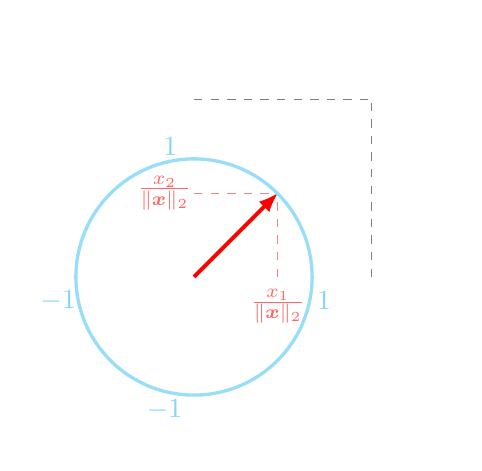
\begin{tikzpicture}[scale=1.5]

% Axes
\draw[->,line width=0.7, white] (-1.4,0)--(1.9,0) node[right]{$x$};
\draw[->,line width=0.7, white] (0,-1.4)--(0,1.8) node[above]{$y$};

% Vectors and dashed lines
\draw[arrows=->, line width=1.2, white] (0,0)--(1.5,1.5);
\draw[dashed, color=gray, thin] (1.5,0)--(1.5,1.5);
\draw[dashed, color=gray, thin] (0,1.5)--(1.5,1.5);

\draw[arrows=->, line width=1.4, color=red] (0,0)--(0.71,0.71);
\draw[dashed, color=red!50, thin] (0.71,0)--(0.71,0.71);
\draw[dashed, color=red!50, thin] (0,0.71)--(0.71,0.71);

% Unit circle
\draw[fill=none, color=cyan!40, line width=1.2] (0,0) circle (1);

% Labels
\node[color=white] at (1.5,-0.15) {$x_1$};
\node[color=white] at (-0.2,1.5) {$x_2$};
\node[color=red!60] at (0.71,-0.25) {$\frac{x_1}{\|\boldsymbol{x}\|_2}$};
\node[color=red!60] at (-0.25,0.71) {$\frac{x_2}{\|\boldsymbol{x}\|_2}$};
\node[color=white] at (1.6,1.6) {$\boldsymbol{x}$};

\node[color=cyan!50] at (1.1,-0.2) {$1$};
\node[color=cyan!50] at (-1.15,-0.2) {$-1$};
\node[color=cyan!50] at (-0.2,1.1) {$1$};
\node[color=cyan!50] at (-0.25,-1.12) {$-1$};

\end{tikzpicture}

\end{document}
